  \section{Monitoring}
    \subsection{Qu'est-ce que c'est ?}
      \bframe
        \begin{itemize}
          \item étude bas niveau du comportement matériel et système
          \item très utile pour le débugage ou l'optimisation poussée
          \item différentes solutions de monitoring existent
	  \begin{itemize}
		\item outils en mode utilisateur
		\item<2-> Performance Monitoring Counters
		\item<3-> Instruction Based Sampling (IBS)
	  \end{itemize}
        \end{itemize}
      \end{frame}

    \subsection{Instruction Based Sampling - Présentation}
      \bframe
        \begin{itemize}
          \item technologie AMD
          \item informations plus précises car IBS spécifique à une famille de
            processeur
          \item problème: plus difficile à mettre en place
        \end{itemize}
      \end{frame}

    \subsection{Instruction Based Sampling - Fonctionnement}
      \bframe
	Principe : 
        \begin{itemize}
          \item taguer aléatoirement une instruction (découpage des instructions)
          \item suivi de l'exécution
          \item deux types de mesures: fetch/execution sampling
        \end{itemize}
      \end{frame}

    \subsection{Instruction Based Sampling - Utilisation}
      \bframe
        \begin{itemize}
          \item<1-2> beaucoup d'informations remontées par IBS
          \item<1-2> sélection des plus utiles: cache hit/miss
	  \item informations stockées dans des registres MSR
        \end{itemize}

        \visible<2->{
          \begin{figure}[h]
            \centering
            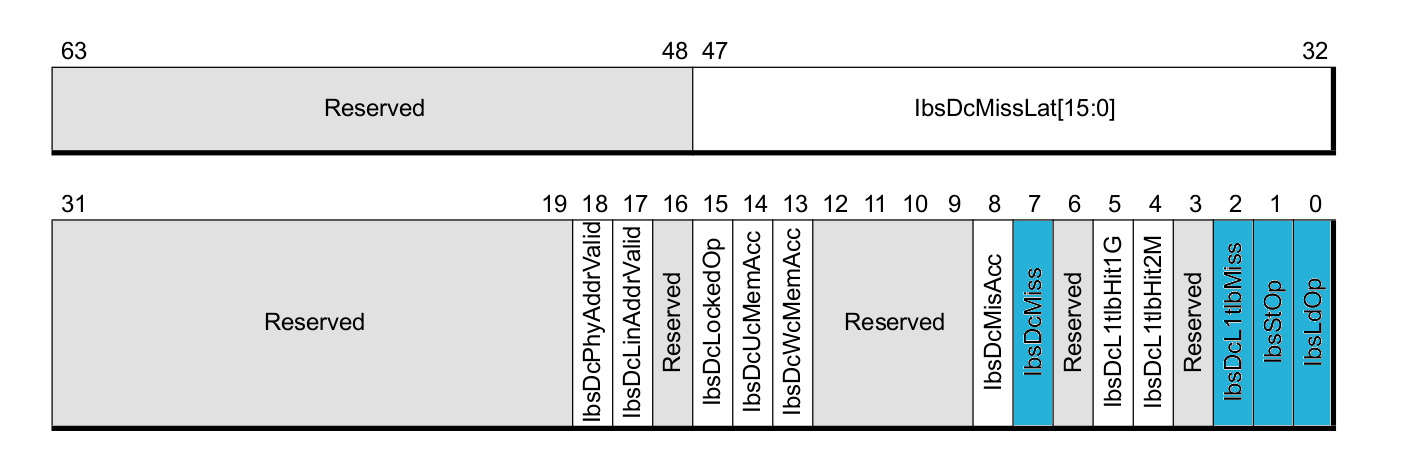
\includegraphics[scale=0.22]{img/data3_color.png}
            \caption{Schéma du registre MSR IbsOpData3}
          \end{figure}
        }
      \end{frame}

   \subsection{Mise en place}
       \begin{frame}{\secname}{\subsecname(1)}        
	\begin{itemize}
 
	  \item les interruptions matérielles - APIC
	  \visible{
            \begin{figure}[h]
              \centering
              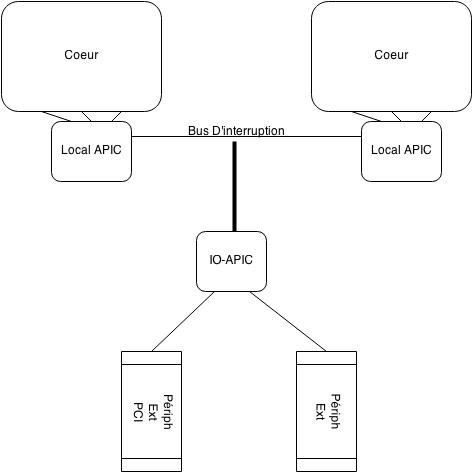
\includegraphics[scale=0.28]{img/apic_diag.jpg}
              \caption{Schéma des composants matériels qui gèrent les interruptions}
            \end{figure}
          }
	  \item<2-> interruptions IBS sont de type NMI (Non Maskable Interrupt)
	\end{itemize}
       \end{frame}

     \begin{frame}{\secname}{\subsecname (2)}        
	Pour configurer les mesures :
	\begin{itemize}
          \item configuration de l'APIC
          \begin{itemize}
            \item informer l'APIC de la présence d'interruptions IBS
            \item à faire pour chaque coeur
          \end{itemize}
          \item enregistrement d'un handler NMI
          \begin{itemize}
            \item appelé à chaque interruption IBS
            \item récolte les informations dans les registres MSR
          \end{itemize}
        \end{itemize}
      \end{frame}


      \begin{frame}{\secname}{\subsecname(3)}
        Lancer les mesures (IbsOpCtl) : 
	\begin{itemize}
	  \item configurer le taux d'échantillonnage
	  \item bit IbsOpEn = 1
	  \item à faire sur le coeur du thread concerné
	\end{itemize}
      \end{frame}


     \subsection{Instruction Based Sampling - Défauts}
     \bframe
       \begin{itemize}
         \item overhead: traitement coûteux des mesures
         \item pas de vision d'ensemble
       \end{itemize}
     \end{frame}

